\documentclass[]{article}
\usepackage{lmodern}
\usepackage{amssymb,amsmath}
\usepackage{ifxetex,ifluatex}
\usepackage{fixltx2e} % provides \textsubscript
\ifnum 0\ifxetex 1\fi\ifluatex 1\fi=0 % if pdftex
  \usepackage[T1]{fontenc}
  \usepackage[utf8]{inputenc}
\else % if luatex or xelatex
  \ifxetex
    \usepackage{mathspec}
  \else
    \usepackage{fontspec}
  \fi
  \defaultfontfeatures{Ligatures=TeX,Scale=MatchLowercase}
\fi
% use upquote if available, for straight quotes in verbatim environments
\IfFileExists{upquote.sty}{\usepackage{upquote}}{}
% use microtype if available
\IfFileExists{microtype.sty}{%
\usepackage{microtype}
\UseMicrotypeSet[protrusion]{basicmath} % disable protrusion for tt fonts
}{}
\usepackage[margin=1in]{geometry}
\usepackage{hyperref}
\hypersetup{unicode=true,
            pdftitle={Report},
            pdfauthor={Varad Srivastava},
            pdfborder={0 0 0},
            breaklinks=true}
\urlstyle{same}  % don't use monospace font for urls
\usepackage{color}
\usepackage{fancyvrb}
\newcommand{\VerbBar}{|}
\newcommand{\VERB}{\Verb[commandchars=\\\{\}]}
\DefineVerbatimEnvironment{Highlighting}{Verbatim}{commandchars=\\\{\}}
% Add ',fontsize=\small' for more characters per line
\usepackage{framed}
\definecolor{shadecolor}{RGB}{248,248,248}
\newenvironment{Shaded}{\begin{snugshade}}{\end{snugshade}}
\newcommand{\KeywordTok}[1]{\textcolor[rgb]{0.13,0.29,0.53}{\textbf{#1}}}
\newcommand{\DataTypeTok}[1]{\textcolor[rgb]{0.13,0.29,0.53}{#1}}
\newcommand{\DecValTok}[1]{\textcolor[rgb]{0.00,0.00,0.81}{#1}}
\newcommand{\BaseNTok}[1]{\textcolor[rgb]{0.00,0.00,0.81}{#1}}
\newcommand{\FloatTok}[1]{\textcolor[rgb]{0.00,0.00,0.81}{#1}}
\newcommand{\ConstantTok}[1]{\textcolor[rgb]{0.00,0.00,0.00}{#1}}
\newcommand{\CharTok}[1]{\textcolor[rgb]{0.31,0.60,0.02}{#1}}
\newcommand{\SpecialCharTok}[1]{\textcolor[rgb]{0.00,0.00,0.00}{#1}}
\newcommand{\StringTok}[1]{\textcolor[rgb]{0.31,0.60,0.02}{#1}}
\newcommand{\VerbatimStringTok}[1]{\textcolor[rgb]{0.31,0.60,0.02}{#1}}
\newcommand{\SpecialStringTok}[1]{\textcolor[rgb]{0.31,0.60,0.02}{#1}}
\newcommand{\ImportTok}[1]{#1}
\newcommand{\CommentTok}[1]{\textcolor[rgb]{0.56,0.35,0.01}{\textit{#1}}}
\newcommand{\DocumentationTok}[1]{\textcolor[rgb]{0.56,0.35,0.01}{\textbf{\textit{#1}}}}
\newcommand{\AnnotationTok}[1]{\textcolor[rgb]{0.56,0.35,0.01}{\textbf{\textit{#1}}}}
\newcommand{\CommentVarTok}[1]{\textcolor[rgb]{0.56,0.35,0.01}{\textbf{\textit{#1}}}}
\newcommand{\OtherTok}[1]{\textcolor[rgb]{0.56,0.35,0.01}{#1}}
\newcommand{\FunctionTok}[1]{\textcolor[rgb]{0.00,0.00,0.00}{#1}}
\newcommand{\VariableTok}[1]{\textcolor[rgb]{0.00,0.00,0.00}{#1}}
\newcommand{\ControlFlowTok}[1]{\textcolor[rgb]{0.13,0.29,0.53}{\textbf{#1}}}
\newcommand{\OperatorTok}[1]{\textcolor[rgb]{0.81,0.36,0.00}{\textbf{#1}}}
\newcommand{\BuiltInTok}[1]{#1}
\newcommand{\ExtensionTok}[1]{#1}
\newcommand{\PreprocessorTok}[1]{\textcolor[rgb]{0.56,0.35,0.01}{\textit{#1}}}
\newcommand{\AttributeTok}[1]{\textcolor[rgb]{0.77,0.63,0.00}{#1}}
\newcommand{\RegionMarkerTok}[1]{#1}
\newcommand{\InformationTok}[1]{\textcolor[rgb]{0.56,0.35,0.01}{\textbf{\textit{#1}}}}
\newcommand{\WarningTok}[1]{\textcolor[rgb]{0.56,0.35,0.01}{\textbf{\textit{#1}}}}
\newcommand{\AlertTok}[1]{\textcolor[rgb]{0.94,0.16,0.16}{#1}}
\newcommand{\ErrorTok}[1]{\textcolor[rgb]{0.64,0.00,0.00}{\textbf{#1}}}
\newcommand{\NormalTok}[1]{#1}
\usepackage{graphicx,grffile}
\makeatletter
\def\maxwidth{\ifdim\Gin@nat@width>\linewidth\linewidth\else\Gin@nat@width\fi}
\def\maxheight{\ifdim\Gin@nat@height>\textheight\textheight\else\Gin@nat@height\fi}
\makeatother
% Scale images if necessary, so that they will not overflow the page
% margins by default, and it is still possible to overwrite the defaults
% using explicit options in \includegraphics[width, height, ...]{}
\setkeys{Gin}{width=\maxwidth,height=\maxheight,keepaspectratio}
\IfFileExists{parskip.sty}{%
\usepackage{parskip}
}{% else
\setlength{\parindent}{0pt}
\setlength{\parskip}{6pt plus 2pt minus 1pt}
}
\setlength{\emergencystretch}{3em}  % prevent overfull lines
\providecommand{\tightlist}{%
  \setlength{\itemsep}{0pt}\setlength{\parskip}{0pt}}
\setcounter{secnumdepth}{0}
% Redefines (sub)paragraphs to behave more like sections
\ifx\paragraph\undefined\else
\let\oldparagraph\paragraph
\renewcommand{\paragraph}[1]{\oldparagraph{#1}\mbox{}}
\fi
\ifx\subparagraph\undefined\else
\let\oldsubparagraph\subparagraph
\renewcommand{\subparagraph}[1]{\oldsubparagraph{#1}\mbox{}}
\fi

%%% Use protect on footnotes to avoid problems with footnotes in titles
\let\rmarkdownfootnote\footnote%
\def\footnote{\protect\rmarkdownfootnote}

%%% Change title format to be more compact
\usepackage{titling}

% Create subtitle command for use in maketitle
\providecommand{\subtitle}[1]{
  \posttitle{
    \begin{center}\large#1\end{center}
    }
}

\setlength{\droptitle}{-2em}

  \title{Report}
    \pretitle{\vspace{\droptitle}\centering\huge}
  \posttitle{\par}
    \author{Varad Srivastava}
    \preauthor{\centering\large\emph}
  \postauthor{\par}
      \predate{\centering\large\emph}
  \postdate{\par}
    \date{March 21, 2019}


\begin{document}
\maketitle

\section{Analysis of Industries :}\label{analysis-of-industries}

\subsection{1. No. of Industries :}\label{no.-of-industries}

Source : Zila Spider Report
(\url{http://updes.up.nic.in/spiderreports/industryReports.jsp}) Talika
35 and 36

\paragraph{Let's take as input the raw
data.}\label{lets-take-as-input-the-raw-data.}

\begin{Shaded}
\begin{Highlighting}[]
\NormalTok{data <-}\StringTok{ }\KeywordTok{read.csv}\NormalTok{(}\StringTok{"data_files/no_of_industries.csv"}\NormalTok{, }\DataTypeTok{header =} \OtherTok{TRUE}\NormalTok{)}
\end{Highlighting}
\end{Shaded}

\paragraph{Visualizing the data:}\label{visualizing-the-data}

Using box plot :
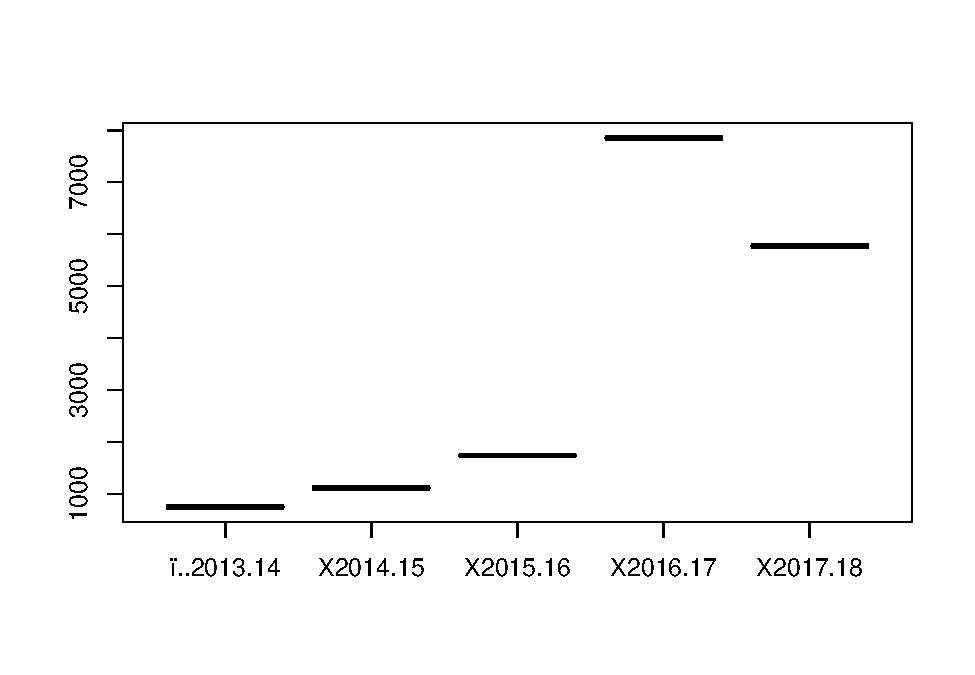
\includegraphics{Report_files/figure-latex/unnamed-chunk-2-1.pdf}

Using Histogram/Bar Chart:
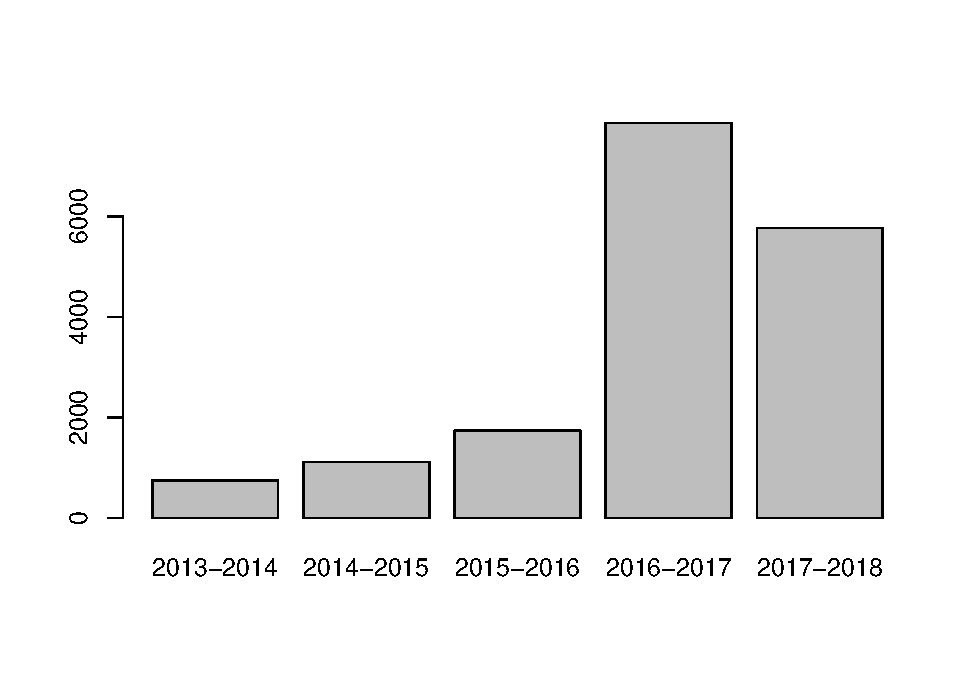
\includegraphics{Report_files/figure-latex/unnamed-chunk-3-1.pdf}

\paragraph{Analysis of Data:}\label{analysis-of-data}

Summary of data:

\begin{verbatim}
##    ï..2013.14     X2014.15       X2015.16       X2016.17       X2017.18   
##  Min.   :744   Min.   :1118   Min.   :1738   Min.   :7855   Min.   :5768  
##  1st Qu.:744   1st Qu.:1118   1st Qu.:1738   1st Qu.:7855   1st Qu.:5768  
##  Median :744   Median :1118   Median :1738   Median :7855   Median :5768  
##  Mean   :744   Mean   :1118   Mean   :1738   Mean   :7855   Mean   :5768  
##  3rd Qu.:744   3rd Qu.:1118   3rd Qu.:1738   3rd Qu.:7855   3rd Qu.:5768  
##  Max.   :744   Max.   :1118   Max.   :1738   Max.   :7855   Max.   :5768
\end{verbatim}

\subsubsection{\texorpdfstring{\textbf{Conclusion} : No. of industuries
have been increasing since the last few years, recording a suprising
jump, in 2016-17, possibily due to ease of doing business. Also to be
noted is that, after 2016-17, no. of industries have seen a sudden
decline, possibly due to cash crunch due to
demonetisation.}{Conclusion : No. of industuries have been increasing since the last few years, recording a suprising jump, in 2016-17, possibily due to ease of doing business. Also to be noted is that, after 2016-17, no. of industries have seen a sudden decline, possibly due to cash crunch due to demonetisation.}}\label{conclusion-no.-of-industuries-have-been-increasing-since-the-last-few-years-recording-a-suprising-jump-in-2016-17-possibily-due-to-ease-of-doing-business.-also-to-be-noted-is-that-after-2016-17-no.-of-industries-have-seen-a-sudden-decline-possibly-due-to-cash-crunch-due-to-demonetisation.}

\subsection{2a. Types of Industries according to labour
:}\label{a.-types-of-industries-according-to-labour}

Source : Zila Spider Report
(\url{http://updes.up.nic.in/spiderreports/industryReports.jsp}) Talika
37

\paragraph{Let's take as input the raw
data.}\label{lets-take-as-input-the-raw-data.-1}

\begin{Shaded}
\begin{Highlighting}[]
\NormalTok{data <-}\StringTok{ }\KeywordTok{read.csv}\NormalTok{(}\StringTok{"data_files/industries_labour.csv"}\NormalTok{, }\DataTypeTok{header =} \OtherTok{TRUE}\NormalTok{)}
\NormalTok{data <-}\StringTok{ }\KeywordTok{cbind}\NormalTok{(}\DataTypeTok{Years =} \KeywordTok{c}\NormalTok{(}\StringTok{"2017-18"}\NormalTok{,}\StringTok{"2016-17"}\NormalTok{,}\StringTok{"2015-16"}\NormalTok{), data)}
\end{Highlighting}
\end{Shaded}

\paragraph{Visualizing the data:}\label{visualizing-the-data-1}

Using box plot :

Using Histogram/Bar Chart:
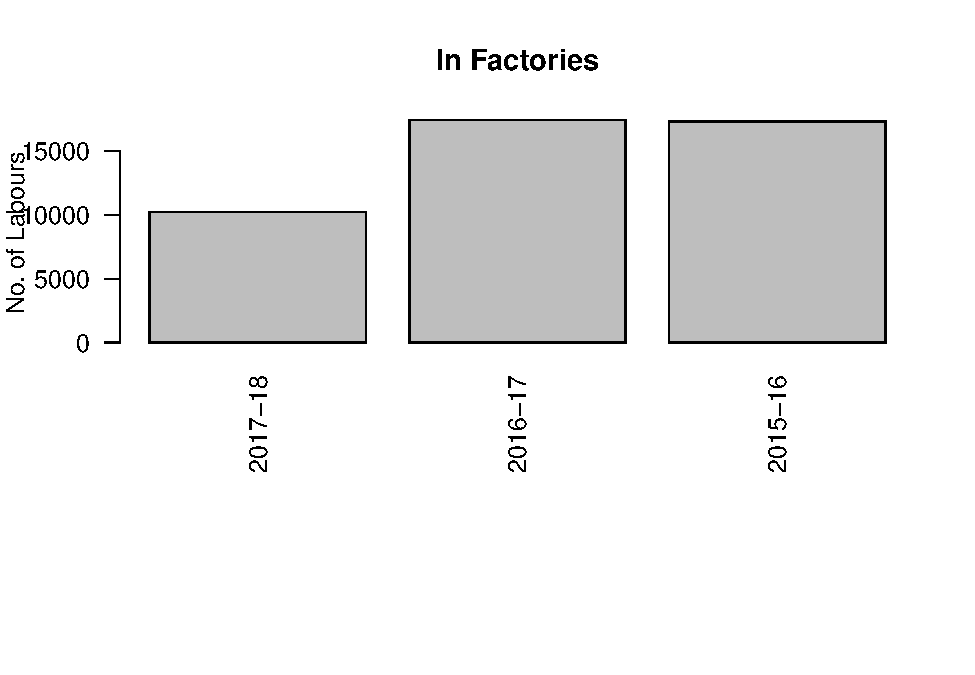
\includegraphics{Report_files/figure-latex/unnamed-chunk-7-1.pdf}
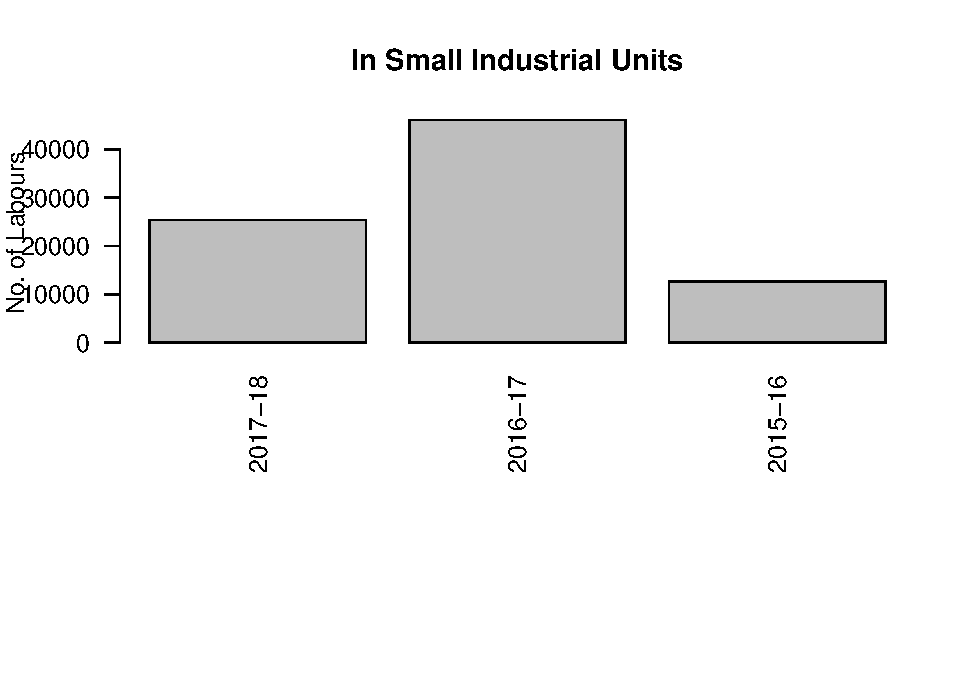
\includegraphics{Report_files/figure-latex/unnamed-chunk-7-2.pdf}
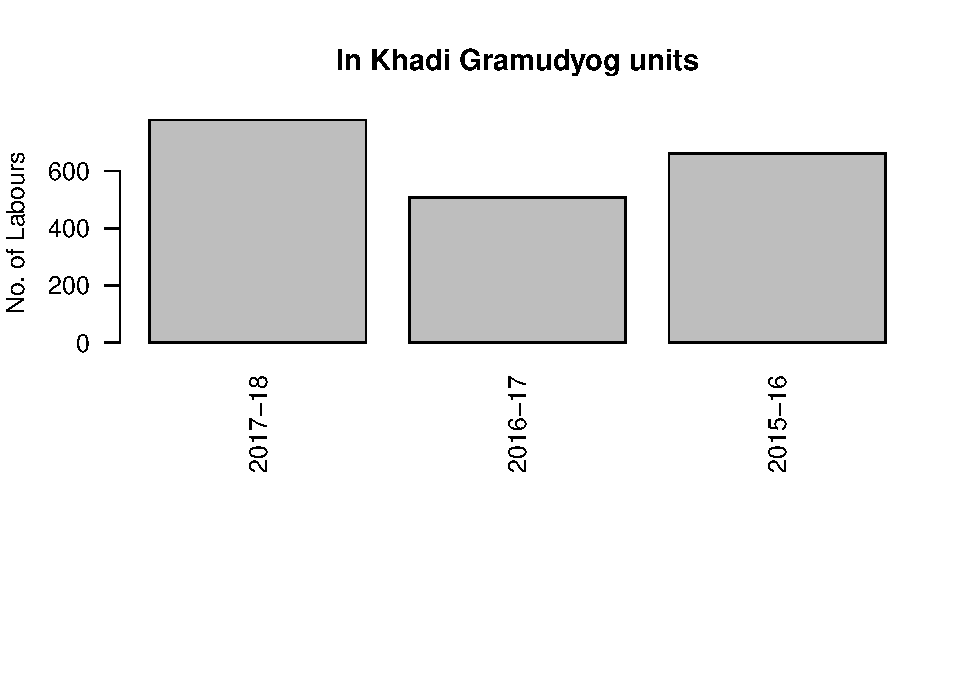
\includegraphics{Report_files/figure-latex/unnamed-chunk-7-3.pdf}

\paragraph{Analysis of Data:}\label{analysis-of-data-1}

Summary of data:

\begin{verbatim}
##      Years    ï..Factories   Small.Industrial.Units Khadi.Gramudyog.units
##  2015-16:1   Min.   :10229   Min.   :12661          Min.   :508.0        
##  2016-17:1   1st Qu.:13781   1st Qu.:19018          1st Qu.:584.5        
##  2017-18:1   Median :17333   Median :25375          Median :661.0        
##              Mean   :14999   Mean   :28027          Mean   :649.0        
##              3rd Qu.:17385   3rd Qu.:35711          3rd Qu.:719.5        
##              Max.   :17436   Max.   :46046          Max.   :778.0
\end{verbatim}

\subsubsection{\texorpdfstring{\textbf{Conclusion} : Most growth has
been witnessed in Khadi Gramudyog units and in small industrial units,
possibily indicating a shift to smaller units, maybe because of
government's initiatives to build up entrpreneruship
avenues.}{Conclusion : Most growth has been witnessed in Khadi Gramudyog units and in small industrial units, possibily indicating a shift to smaller units, maybe because of government's initiatives to build up entrpreneruship avenues.}}\label{conclusion-most-growth-has-been-witnessed-in-khadi-gramudyog-units-and-in-small-industrial-units-possibily-indicating-a-shift-to-smaller-units-maybe-because-of-governments-initiatives-to-build-up-entrpreneruship-avenues.}

\subsection{2c. Types of Industries according to Ownership
:}\label{c.-types-of-industries-according-to-ownership}

Source : Zila Spider Report
(\url{http://updes.up.nic.in/spiderreports/industryReports.jsp}) Talika
36

\paragraph{Let's take as input the raw
data.}\label{lets-take-as-input-the-raw-data.-2}

\begin{Shaded}
\begin{Highlighting}[]
\NormalTok{data <-}\StringTok{ }\KeywordTok{read.csv}\NormalTok{(}\StringTok{"data_files/industries_ownership.csv"}\NormalTok{, }\DataTypeTok{header =} \OtherTok{TRUE}\NormalTok{)}
\end{Highlighting}
\end{Shaded}

\paragraph{Visualizing the data:}\label{visualizing-the-data-2}

Using box plot :
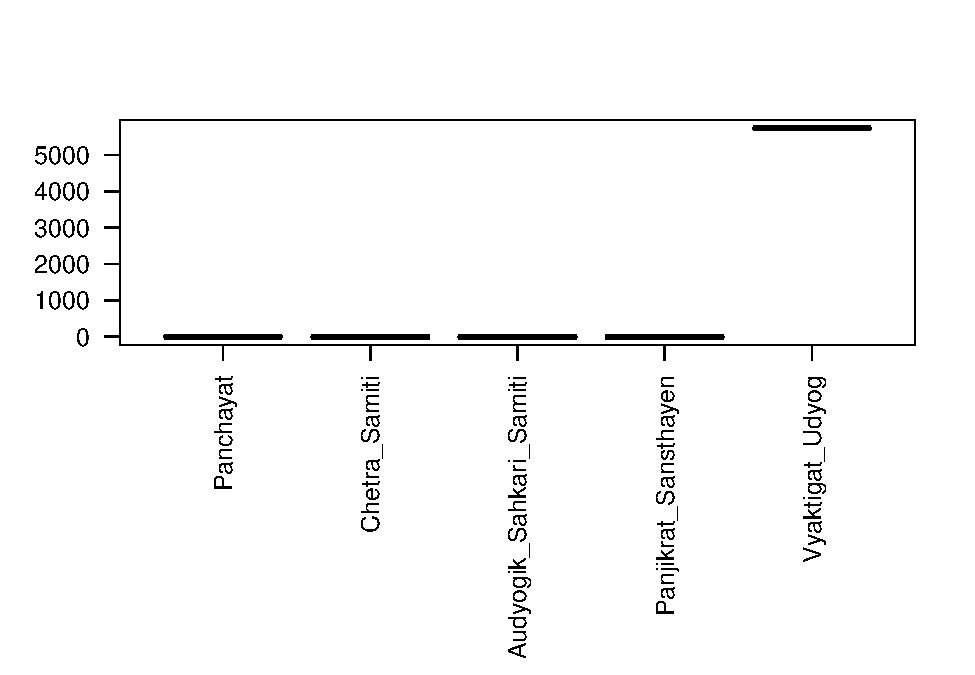
\includegraphics{Report_files/figure-latex/unnamed-chunk-10-1.pdf}

Using Histogram/Bar Chart:
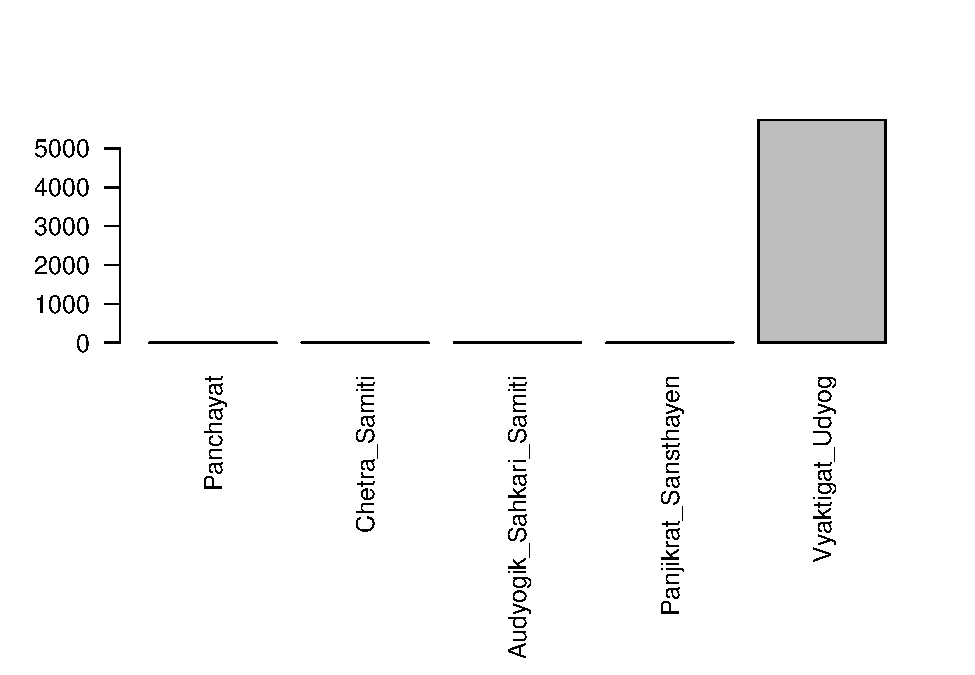
\includegraphics{Report_files/figure-latex/unnamed-chunk-11-1.pdf}

\paragraph{Analysis of Data:}\label{analysis-of-data-2}

Summary of data:

\begin{verbatim}
##   ï..Panchayat Chetra.Samiti Auduogik.Sahkari.Samiti Panjikrat.Sansthayen
##  Min.   :0     Min.   :0     Min.   :0               Min.   :0           
##  1st Qu.:0     1st Qu.:0     1st Qu.:0               1st Qu.:0           
##  Median :0     Median :0     Median :0               Median :0           
##  Mean   :0     Mean   :0     Mean   :0               Mean   :0           
##  3rd Qu.:0     3rd Qu.:0     3rd Qu.:0               3rd Qu.:0           
##  Max.   :0     Max.   :0     Max.   :0               Max.   :0           
##  Vyaktigat.Udyog
##  Min.   :5730   
##  1st Qu.:5730   
##  Median :5730   
##  Mean   :5730   
##  3rd Qu.:5730   
##  Max.   :5730
\end{verbatim}

\subsubsection{\texorpdfstring{\textbf{Conclusion} : No. of industuries,
belonging to Panchayat, Chetra Samiti, Adyogik Sahkari Samiti and
Panjikrat Sansthayen are virtually 0. Although, the industries owned by
individuals, i.e.~Vyaktigat Udyog, are on the rise, can ring some bells
of happiness ,signaling an increase in entrepreneurship, still, these
are worrysome figures, and more focus is needed on industries owned by
cooperatives and Panchayats, so that village people can be empowered as
well.}{Conclusion : No. of industuries, belonging to Panchayat, Chetra Samiti, Adyogik Sahkari Samiti and Panjikrat Sansthayen are virtually 0. Although, the industries owned by individuals, i.e.~Vyaktigat Udyog, are on the rise, can ring some bells of happiness ,signaling an increase in entrepreneurship, still, these are worrysome figures, and more focus is needed on industries owned by cooperatives and Panchayats, so that village people can be empowered as well.}}\label{conclusion-no.-of-industuries-belonging-to-panchayat-chetra-samiti-adyogik-sahkari-samiti-and-panjikrat-sansthayen-are-virtually-0.-although-the-industries-owned-by-individuals-i.e.vyaktigat-udyog-are-on-the-rise-can-ring-some-bells-of-happiness-signaling-an-increase-in-entrepreneurship-still-these-are-worrysome-figures-and-more-focus-is-needed-on-industries-owned-by-cooperatives-and-panchayats-so-that-village-people-can-be-empowered-as-well.}

\section{Analysis of Electricity}\label{analysis-of-electricity}

\subsection{No. Electricity connections in rural areas
:}\label{no.-electricity-connections-in-rural-areas}

Source : Zila Spider Report
(\url{http://updes.up.nic.in/spiderreports/gettable48Report.action})
Talika 48

\paragraph{Let's take as input the raw
data.}\label{lets-take-as-input-the-raw-data.-3}

\begin{Shaded}
\begin{Highlighting}[]
\NormalTok{data <-}\StringTok{ }\KeywordTok{read.csv}\NormalTok{(}\StringTok{"data_files/electric_connections.csv"}\NormalTok{, }\DataTypeTok{header =} \OtherTok{TRUE}\NormalTok{)}
\end{Highlighting}
\end{Shaded}

\paragraph{Visualizing the data:}\label{visualizing-the-data-3}

Using box plot :
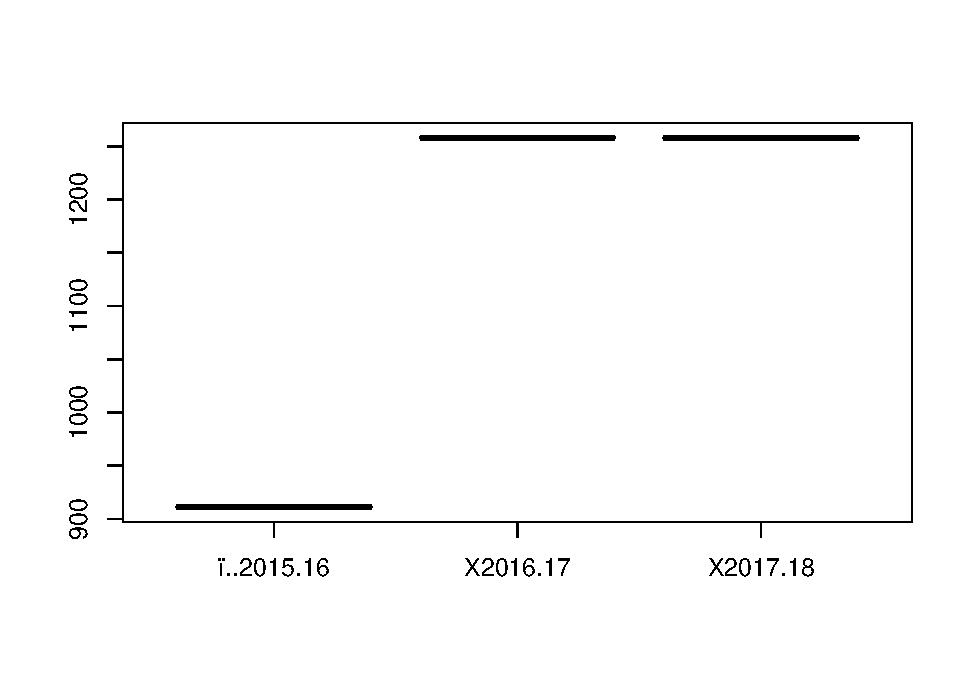
\includegraphics{Report_files/figure-latex/unnamed-chunk-14-1.pdf}

Using Histogram/Bar Chart:
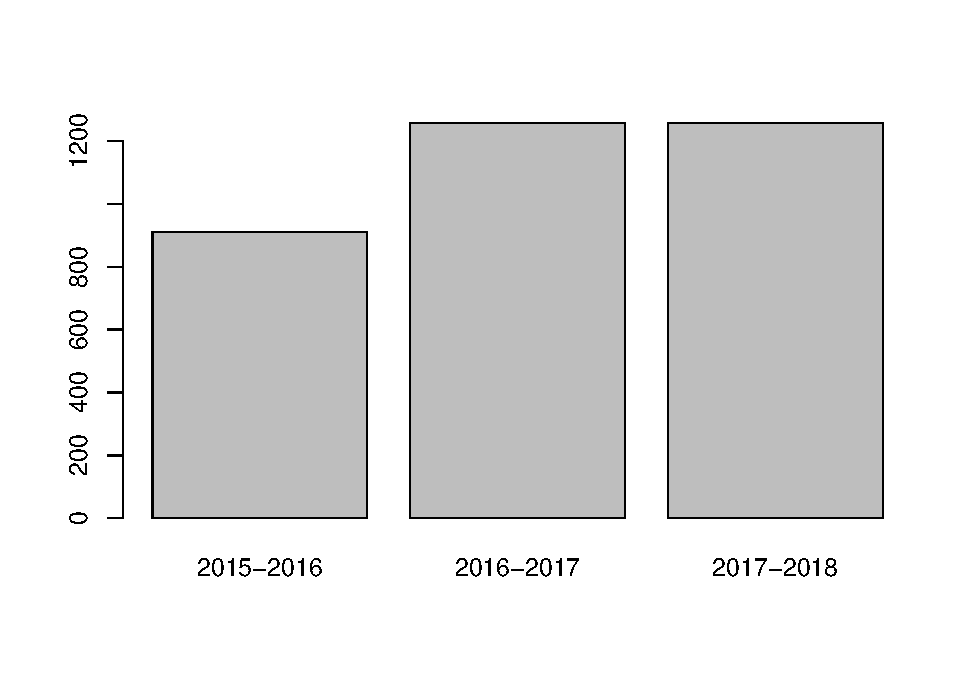
\includegraphics{Report_files/figure-latex/unnamed-chunk-15-1.pdf}

\paragraph{Analysis of Data:}\label{analysis-of-data-3}

Summary of data:

\begin{verbatim}
##    ï..2015.16     X2016.17       X2017.18   
##  Min.   :911   Min.   :1258   Min.   :1258  
##  1st Qu.:911   1st Qu.:1258   1st Qu.:1258  
##  Median :911   Median :1258   Median :1258  
##  Mean   :911   Mean   :1258   Mean   :1258  
##  3rd Qu.:911   3rd Qu.:1258   3rd Qu.:1258  
##  Max.   :911   Max.   :1258   Max.   :1258
\end{verbatim}

\subsubsection{\texorpdfstring{\textbf{Conclusion} : No. of electric
connections have been steadly increasing since the last few years,
possibily due to government's new schemes like Pradhan Mantri Sahaj
Bijli Har Ghar
Yojana.}{Conclusion : No. of electric connections have been steadly increasing since the last few years, possibily due to government's new schemes like Pradhan Mantri Sahaj Bijli Har Ghar Yojana.}}\label{conclusion-no.-of-electric-connections-have-been-steadly-increasing-since-the-last-few-years-possibily-due-to-governments-new-schemes-like-pradhan-mantri-sahaj-bijli-har-ghar-yojana.}

\section{Analysis of Education}\label{analysis-of-education}

\subsection{No. schools, colleges and universities
:}\label{no.-schools-colleges-and-universities}

Source : Zila Spider Report
(\url{http://updes.up.nic.in/spiderreports/gettable39Report.action})
Talika 39

\paragraph{Let's take as input the raw
data.}\label{lets-take-as-input-the-raw-data.-4}

\begin{Shaded}
\begin{Highlighting}[]
\NormalTok{data <-}\StringTok{ }\KeywordTok{read.csv}\NormalTok{(}\StringTok{"data_files/education_nos.csv"}\NormalTok{, }\DataTypeTok{header =} \OtherTok{TRUE}\NormalTok{)}
\end{Highlighting}
\end{Shaded}

\paragraph{Visualizing the data:}\label{visualizing-the-data-4}

Using box plot :
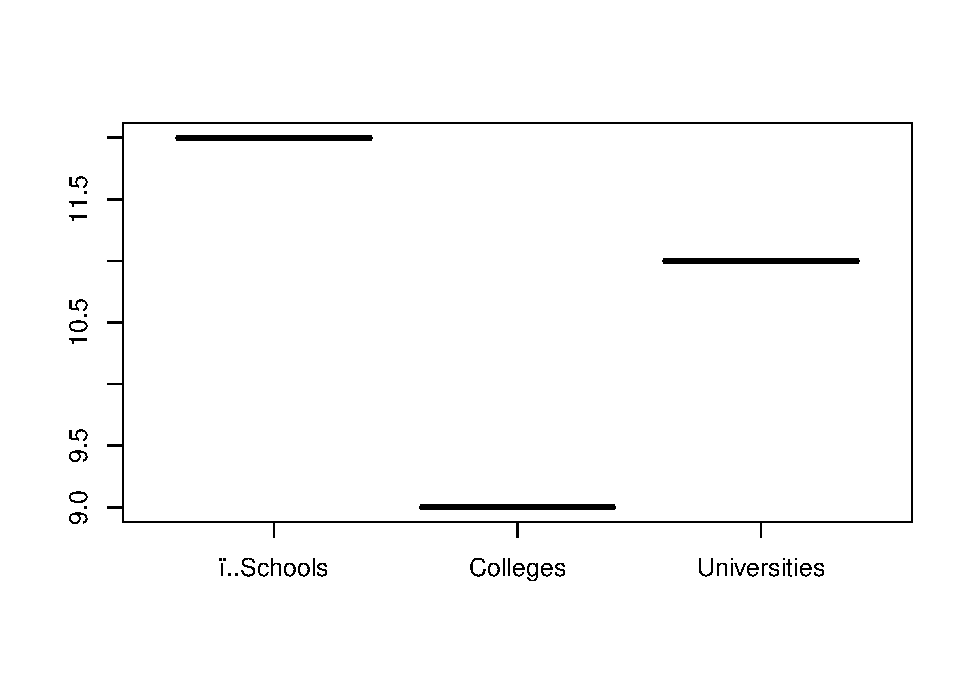
\includegraphics{Report_files/figure-latex/unnamed-chunk-18-1.pdf}

Using Histogram/Bar Chart:
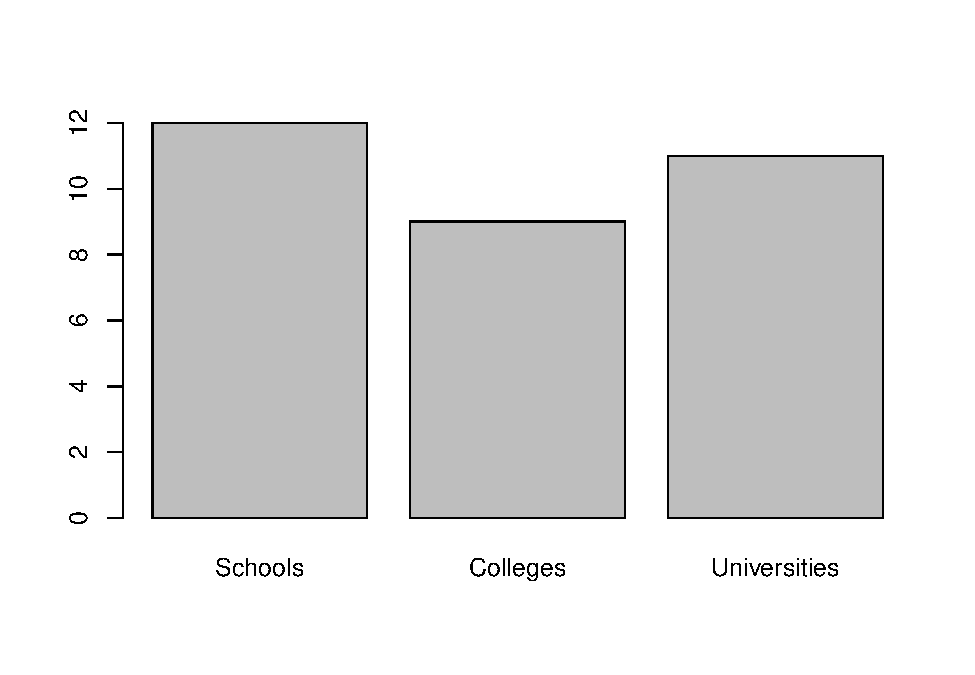
\includegraphics{Report_files/figure-latex/unnamed-chunk-19-1.pdf}

\paragraph{Analysis of Data:}\label{analysis-of-data-4}

Summary of data:

\begin{verbatim}
##    ï..Schools    Colleges  Universities
##  Min.   :12   Min.   :9   Min.   :11   
##  1st Qu.:12   1st Qu.:9   1st Qu.:11   
##  Median :12   Median :9   Median :11   
##  Mean   :12   Mean   :9   Mean   :11   
##  3rd Qu.:12   3rd Qu.:9   3rd Qu.:11   
##  Max.   :12   Max.   :9   Max.   :11
\end{verbatim}

\subsubsection{\texorpdfstring{\textbf{Conclusion} : No. of educational
institutions are significant in the district, with the presence of even
notable institutions like BHU and IIT. However,much can be done on the
front of colleges and schools. With the district population growing as a
fast pace, with the influx of rural population from nearby villages,
necessity for more schools and colleges is going to
increase.}{Conclusion : No. of educational institutions are significant in the district, with the presence of even notable institutions like BHU and IIT. However,much can be done on the front of colleges and schools. With the district population growing as a fast pace, with the influx of rural population from nearby villages, necessity for more schools and colleges is going to increase.}}\label{conclusion-no.-of-educational-institutions-are-significant-in-the-district-with-the-presence-of-even-notable-institutions-like-bhu-and-iit.-howevermuch-can-be-done-on-the-front-of-colleges-and-schools.-with-the-district-population-growing-as-a-fast-pace-with-the-influx-of-rural-population-from-nearby-villages-necessity-for-more-schools-and-colleges-is-going-to-increase.}

\subsection{No. of teachers :}\label{no.-of-teachers}

Source : Zila Spider Report
(\url{http://updes.up.nic.in/spiderreports/gettable41Report.action})
Talika 41

\paragraph{Let's take as input the raw
data.}\label{lets-take-as-input-the-raw-data.-5}

\begin{Shaded}
\begin{Highlighting}[]
\NormalTok{data <-}\StringTok{ }\KeywordTok{read.csv}\NormalTok{(}\StringTok{"data_files/teachers.csv"}\NormalTok{, }\DataTypeTok{header =} \OtherTok{TRUE}\NormalTok{)}
\end{Highlighting}
\end{Shaded}

\paragraph{Visualizing the data:}\label{visualizing-the-data-5}

Using box plot :
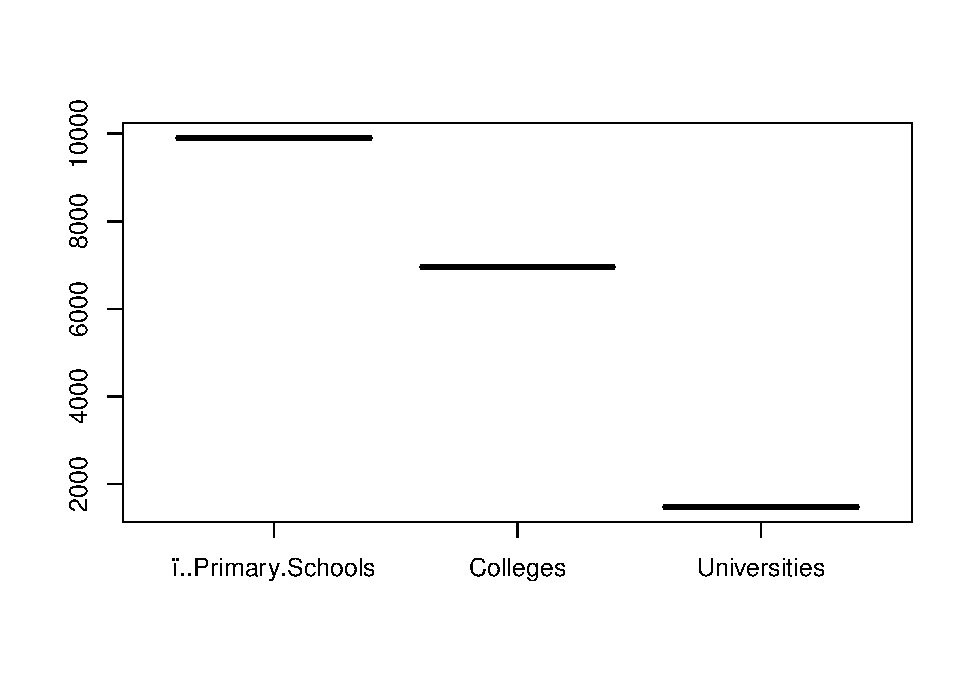
\includegraphics{Report_files/figure-latex/unnamed-chunk-22-1.pdf}

Using Histogram/Bar Chart:
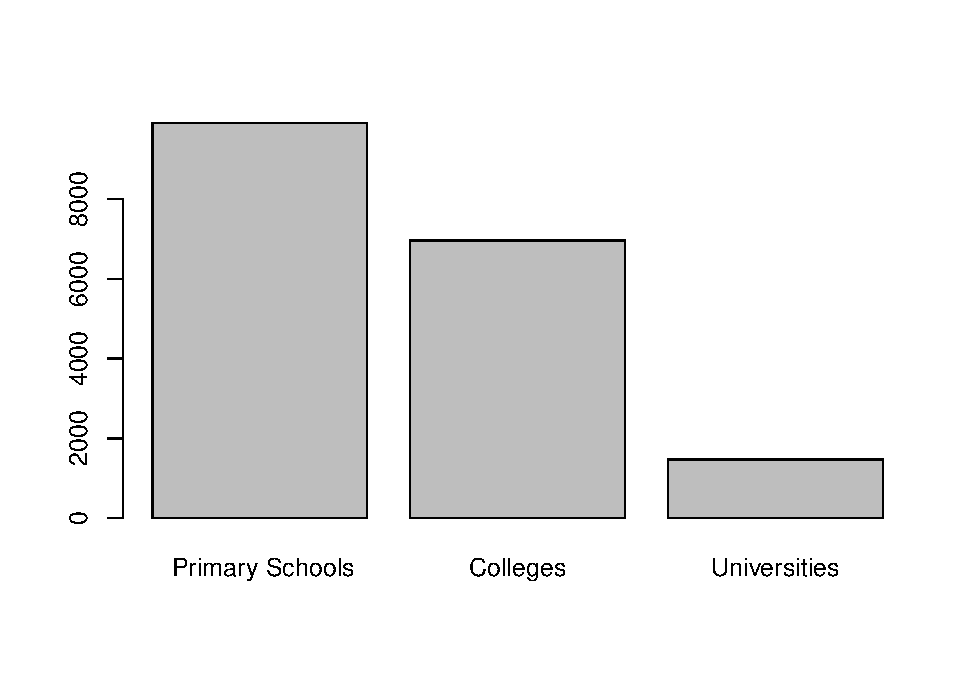
\includegraphics{Report_files/figure-latex/unnamed-chunk-23-1.pdf}

\paragraph{Analysis of Data:}\label{analysis-of-data-5}

Summary of data:

\begin{verbatim}
##  ï..Primary.Schools    Colleges     Universities 
##  Min.   :9908       Min.   :6956   Min.   :1467  
##  1st Qu.:9908       1st Qu.:6956   1st Qu.:1467  
##  Median :9908       Median :6956   Median :1467  
##  Mean   :9908       Mean   :6956   Mean   :1467  
##  3rd Qu.:9908       3rd Qu.:6956   3rd Qu.:1467  
##  Max.   :9908       Max.   :6956   Max.   :1467
\end{verbatim}

\subsubsection{\texorpdfstring{\textbf{Conclusion} : No. of teachers
although show a positive feature, but the quality of education remains
low, indicating, lack of quality, not quantity. The screening process of
teachers need to match the necessities of the modern
world.}{Conclusion : No. of teachers although show a positive feature, but the quality of education remains low, indicating, lack of quality, not quantity. The screening process of teachers need to match the necessities of the modern world.}}\label{conclusion-no.-of-teachers-although-show-a-positive-feature-but-the-quality-of-education-remains-low-indicating-lack-of-quality-not-quantity.-the-screening-process-of-teachers-need-to-match-the-necessities-of-the-modern-world.}

\section{Analysis of Irrigation}\label{analysis-of-irrigation}

\subsection{Irrigation Area :}\label{irrigation-area}

Source : Zila Spider Report
(\url{http://updes.up.nic.in/spiderreports/gettable18Report.action})
Talika 18

\paragraph{Let's take as input the raw
data.}\label{lets-take-as-input-the-raw-data.-6}

\begin{Shaded}
\begin{Highlighting}[]
\NormalTok{data <-}\StringTok{ }\KeywordTok{read.csv}\NormalTok{(}\StringTok{"data_files/irrigation_area.csv"}\NormalTok{, }\DataTypeTok{header =} \OtherTok{TRUE}\NormalTok{)}
\end{Highlighting}
\end{Shaded}

\paragraph{Visualizing the data:}\label{visualizing-the-data-6}

Using box plot :
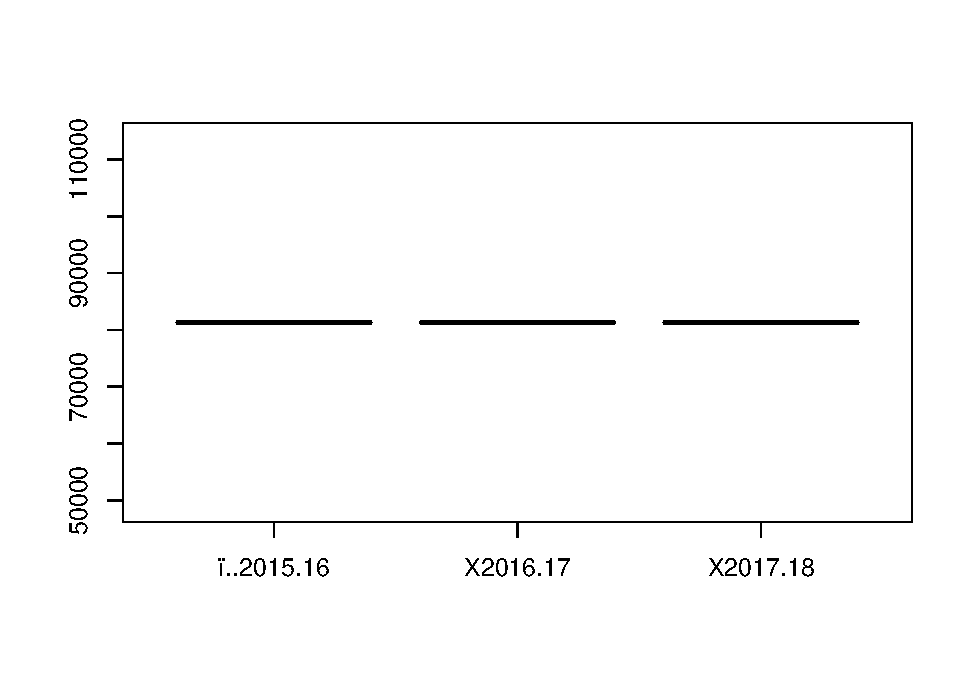
\includegraphics{Report_files/figure-latex/unnamed-chunk-26-1.pdf}

Using Histogram/Bar Chart:
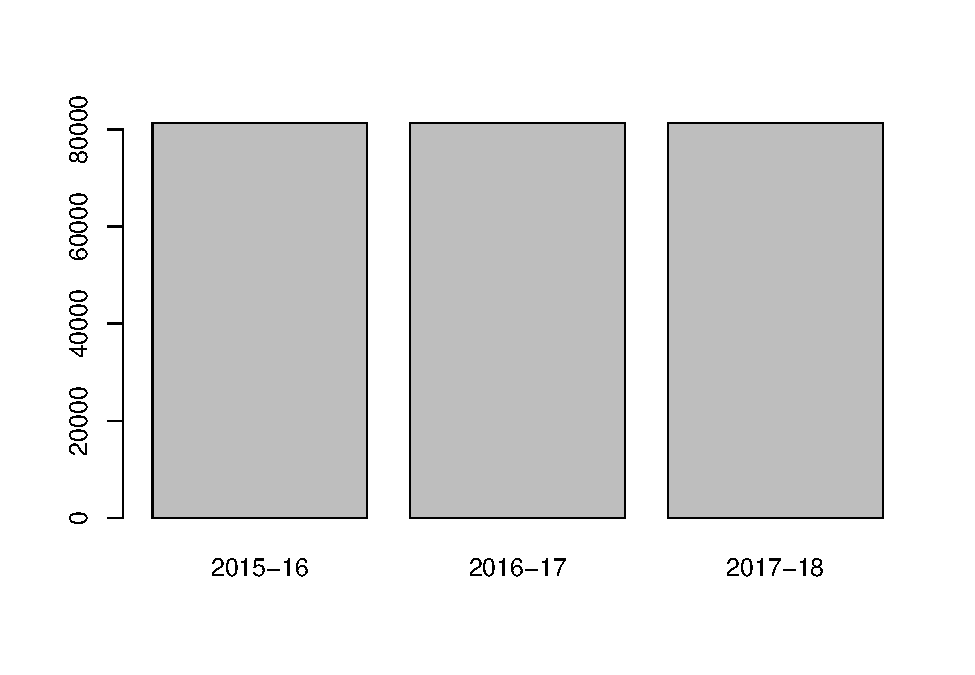
\includegraphics{Report_files/figure-latex/unnamed-chunk-27-1.pdf}

\paragraph{Analysis of Data:}\label{analysis-of-data-6}

Summary of data:

\begin{verbatim}
##    ï..2015.16       X2016.17        X2017.18    
##  Min.   :81319   Min.   :81319   Min.   :81319  
##  1st Qu.:81319   1st Qu.:81319   1st Qu.:81319  
##  Median :81319   Median :81319   Median :81319  
##  Mean   :81319   Mean   :81319   Mean   :81319  
##  3rd Qu.:81319   3rd Qu.:81319   3rd Qu.:81319  
##  Max.   :81319   Max.   :81319   Max.   :81319
\end{verbatim}

\subsubsection{\texorpdfstring{\textbf{Conclusion} : Amount of
irrigation area shows up more or less, over the last three years,
indicating a fault in government
records.}{Conclusion : Amount of irrigation area shows up more or less, over the last three years, indicating a fault in government records.}}\label{conclusion-amount-of-irrigation-area-shows-up-more-or-less-over-the-last-three-years-indicating-a-fault-in-government-records.}

\subsection{Number of canals and ponds
:}\label{number-of-canals-and-ponds}

Source : Zila Spider Report
(\url{http://updes.up.nic.in/spiderreports/gettable18Report.action})
Talika 18

\paragraph{Let's take as input the raw
data.}\label{lets-take-as-input-the-raw-data.-7}

\begin{Shaded}
\begin{Highlighting}[]
\NormalTok{data <-}\StringTok{ }\KeywordTok{read.csv}\NormalTok{(}\StringTok{"data_files/ponds_canals.csv"}\NormalTok{, }\DataTypeTok{header =} \OtherTok{TRUE}\NormalTok{)}
\end{Highlighting}
\end{Shaded}

\paragraph{Visualizing the data:}\label{visualizing-the-data-7}

Using box plot :
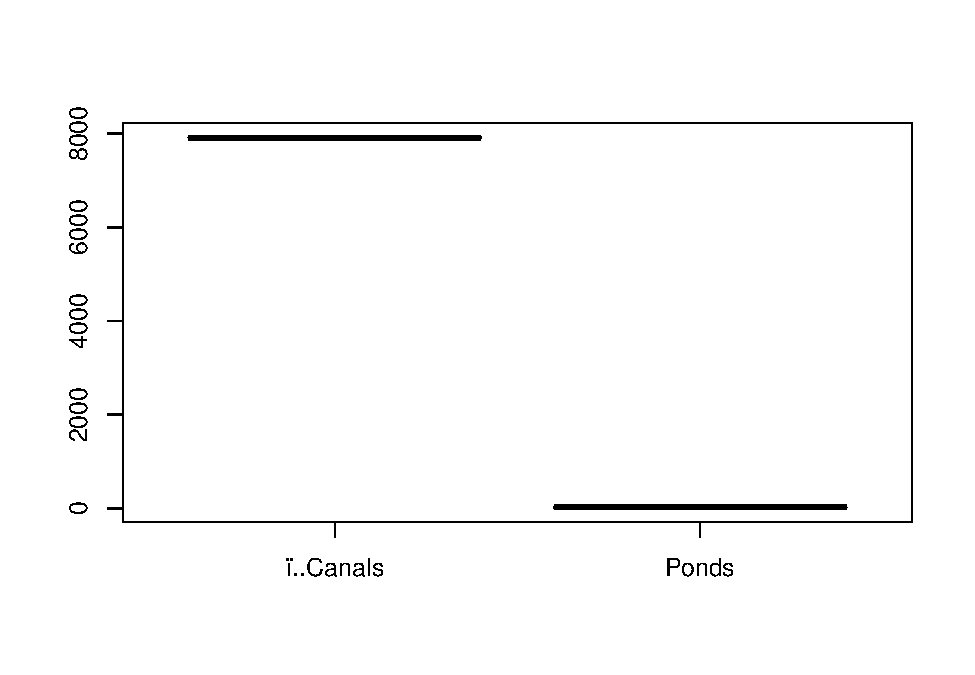
\includegraphics{Report_files/figure-latex/unnamed-chunk-30-1.pdf}

Using Histogram/Bar Chart:
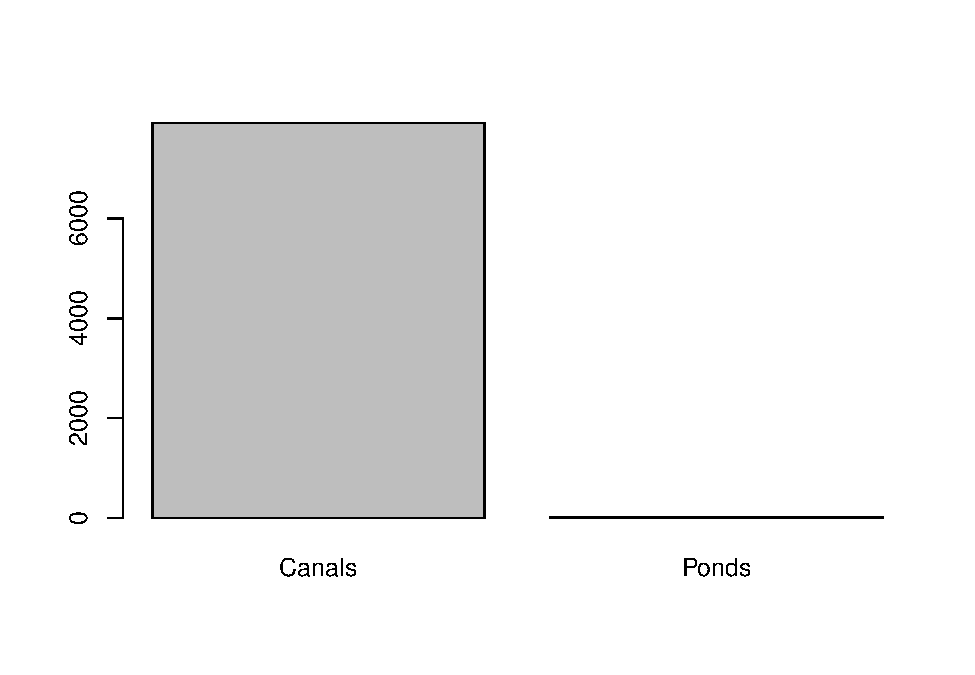
\includegraphics{Report_files/figure-latex/unnamed-chunk-31-1.pdf}

\paragraph{Analysis of Data:}\label{analysis-of-data-7}

Summary of data:

\begin{verbatim}
##    ï..Canals        Ponds   
##  Min.   :7909   Min.   :24  
##  1st Qu.:7909   1st Qu.:24  
##  Median :7909   Median :24  
##  Mean   :7909   Mean   :24  
##  3rd Qu.:7909   3rd Qu.:24  
##  Max.   :7909   Max.   :24
\end{verbatim}

\subsubsection{\texorpdfstring{\textbf{Conclusion} : Number of canals
and ponds in the district are in decent amount in 2018. Although, due to
rapid urbanisation, many ponds are getting depleted
quickly.}{Conclusion : Number of canals and ponds in the district are in decent amount in 2018. Although, due to rapid urbanisation, many ponds are getting depleted quickly.}}\label{conclusion-number-of-canals-and-ponds-in-the-district-are-in-decent-amount-in-2018.-although-due-to-rapid-urbanisation-many-ponds-are-getting-depleted-quickly.}

\subsection{Number of tubewells electric and diesel
:}\label{number-of-tubewells-electric-and-diesel}

Source : Zila Spider Report
(\url{http://updes.up.nic.in/spiderreports/gettable23Report.action})
Talika 23

\paragraph{Let's take as input the raw
data.}\label{lets-take-as-input-the-raw-data.-8}

\begin{Shaded}
\begin{Highlighting}[]
\NormalTok{data1 <-}\StringTok{ }\KeywordTok{read.csv}\NormalTok{(}\StringTok{"data_files/tubewellse.csv"}\NormalTok{, }\DataTypeTok{header =} \OtherTok{TRUE}\NormalTok{)}
\NormalTok{data2 <-}\StringTok{ }\KeywordTok{read.csv}\NormalTok{(}\StringTok{"data_files/tubewellsdiesel.csv"}\NormalTok{, }\DataTypeTok{header =} \OtherTok{TRUE}\NormalTok{)}
\end{Highlighting}
\end{Shaded}

\paragraph{Visualizing the data:}\label{visualizing-the-data-8}

Using box plot :
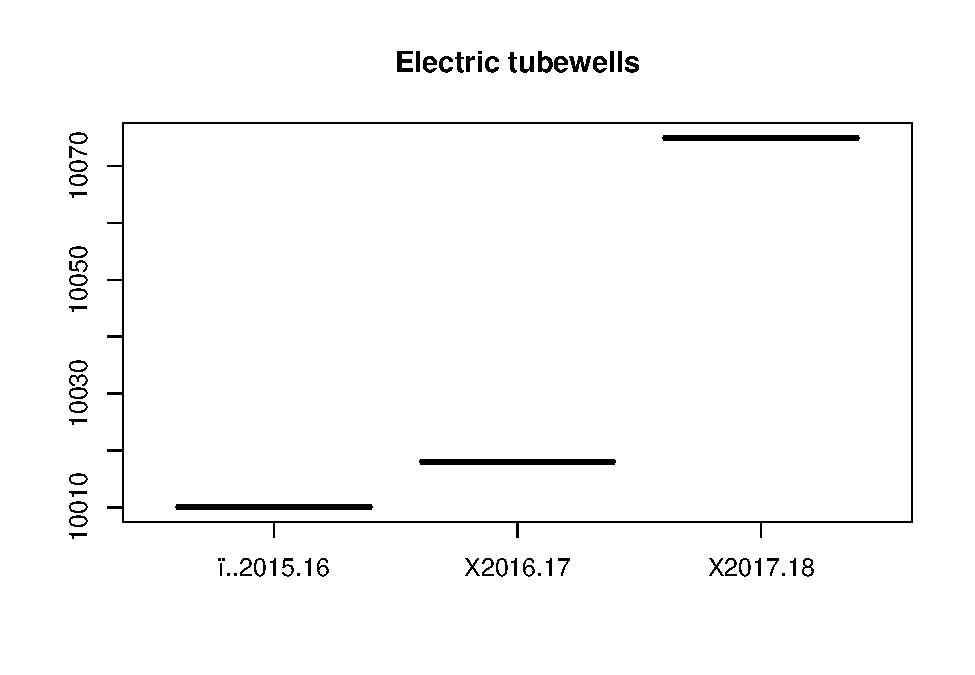
\includegraphics{Report_files/figure-latex/unnamed-chunk-34-1.pdf}
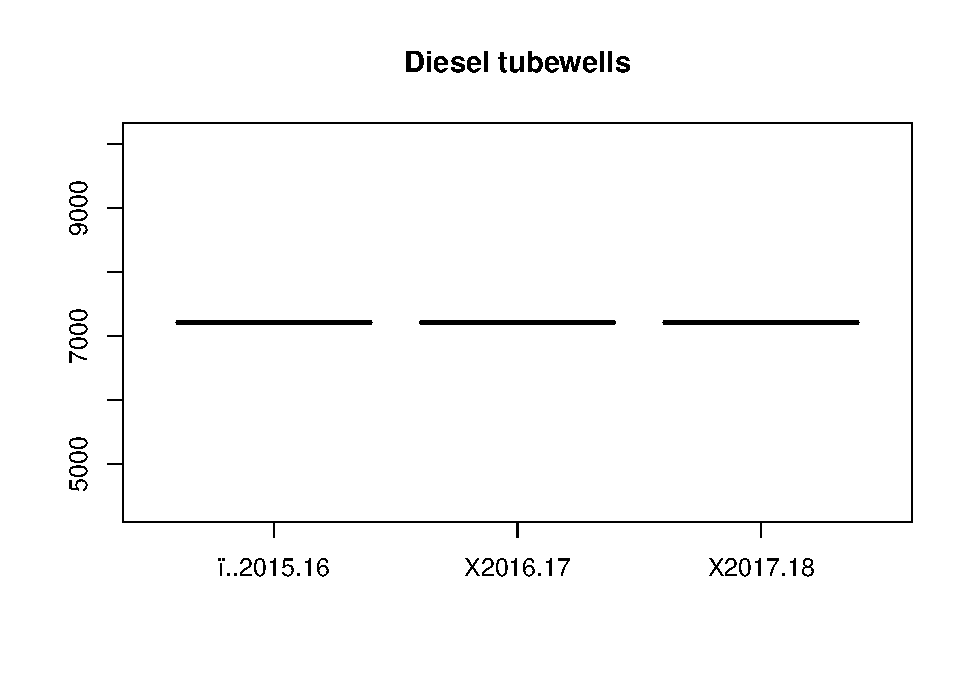
\includegraphics{Report_files/figure-latex/unnamed-chunk-34-2.pdf}

Using Histogram/Bar Chart:
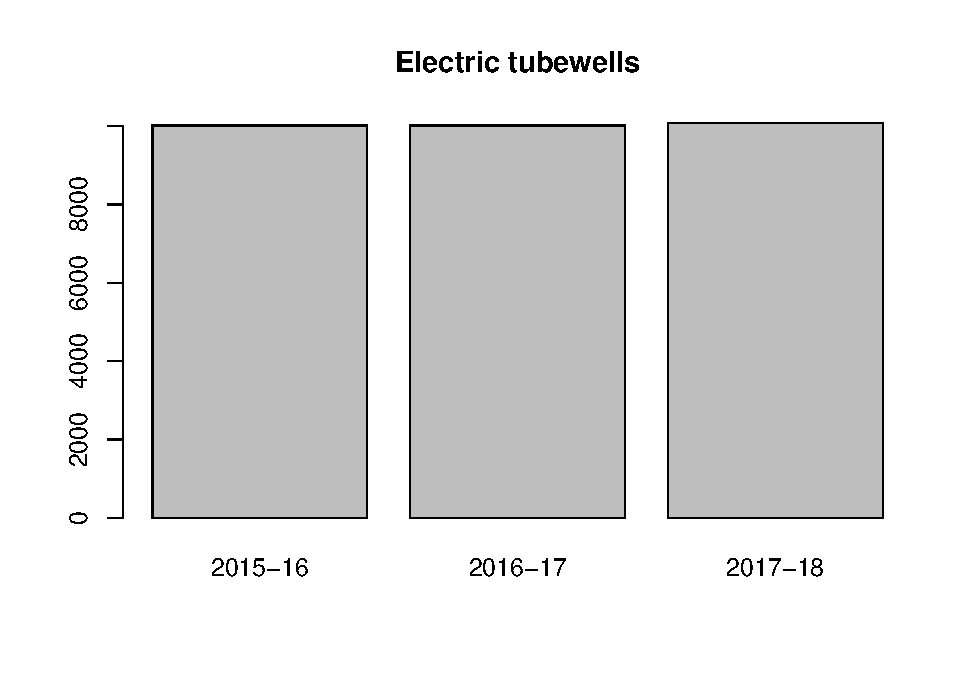
\includegraphics{Report_files/figure-latex/unnamed-chunk-35-1.pdf}
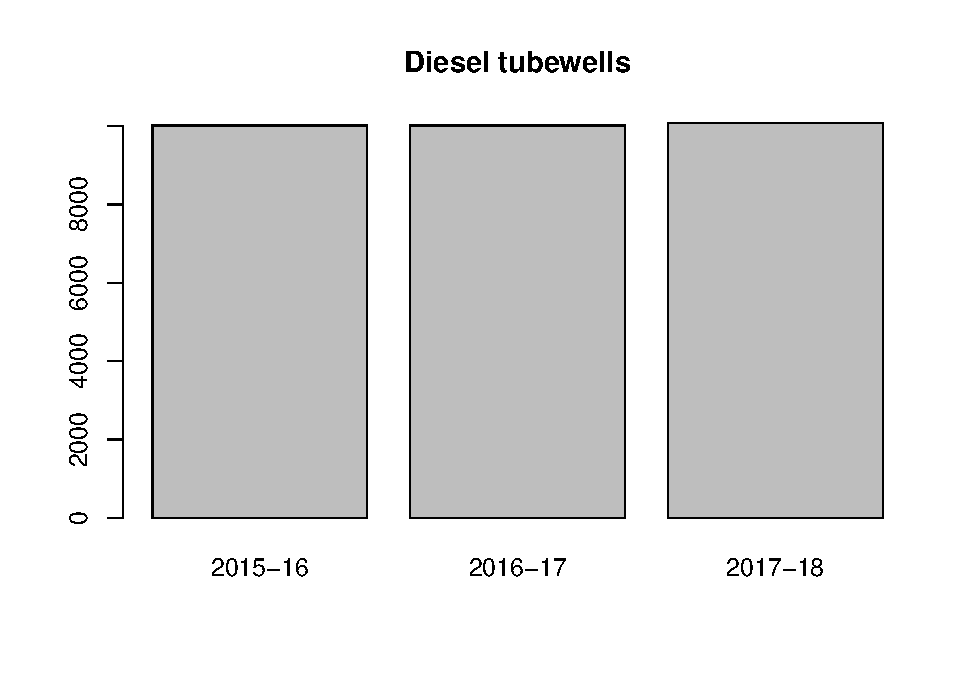
\includegraphics{Report_files/figure-latex/unnamed-chunk-35-2.pdf}

\paragraph{Analysis of Data:}\label{analysis-of-data-8}

Summary of data:

\begin{verbatim}
##    ï..Canals        Ponds   
##  Min.   :7909   Min.   :24  
##  1st Qu.:7909   1st Qu.:24  
##  Median :7909   Median :24  
##  Mean   :7909   Mean   :24  
##  3rd Qu.:7909   3rd Qu.:24  
##  Max.   :7909   Max.   :24
\end{verbatim}

\subsubsection{\texorpdfstring{\textbf{Conclusion} : Number of electric
tubewells have shown a steady increase while stangnant nature of diesel
ones. This is a good sign, as our dependence on crude oil decreases and
it is good for the environment
too.}{Conclusion : Number of electric tubewells have shown a steady increase while stangnant nature of diesel ones. This is a good sign, as our dependence on crude oil decreases and it is good for the environment too.}}\label{conclusion-number-of-electric-tubewells-have-shown-a-steady-increase-while-stangnant-nature-of-diesel-ones.-this-is-a-good-sign-as-our-dependence-on-crude-oil-decreases-and-it-is-good-for-the-environment-too.}

\subsection{Number of borewells :}\label{number-of-borewells}

Source : Zila Spider Report
(\url{http://updes.up.nic.in/spiderreports/gettable23Report.action})
Talika 23

\paragraph{Let's take as input the raw
data.}\label{lets-take-as-input-the-raw-data.-9}

\begin{Shaded}
\begin{Highlighting}[]
\NormalTok{data <-}\StringTok{ }\KeywordTok{read.csv}\NormalTok{(}\StringTok{"data_files/borewells.csv"}\NormalTok{, }\DataTypeTok{header =} \OtherTok{TRUE}\NormalTok{)}
\end{Highlighting}
\end{Shaded}

\paragraph{Visualizing the data:}\label{visualizing-the-data-9}

Using box plot :
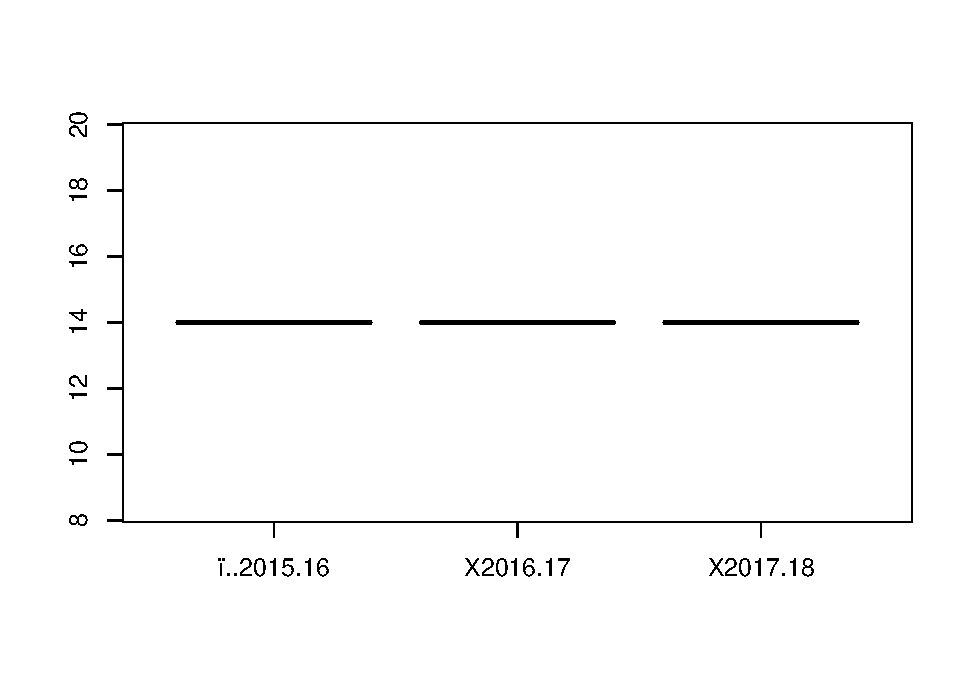
\includegraphics{Report_files/figure-latex/unnamed-chunk-38-1.pdf}

Using Histogram/Bar Chart:
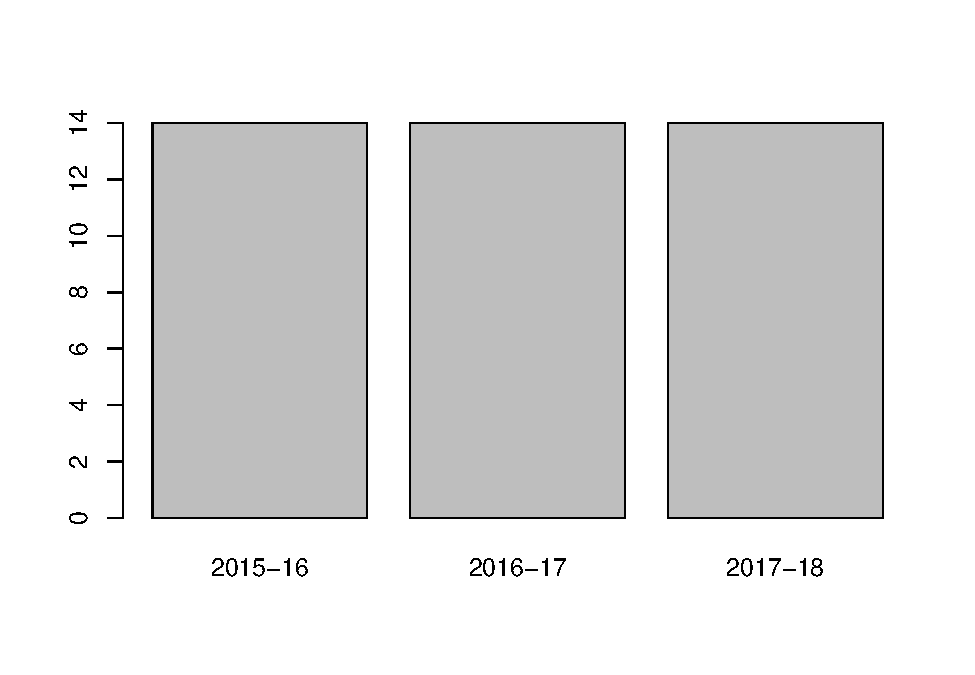
\includegraphics{Report_files/figure-latex/unnamed-chunk-39-1.pdf}

\paragraph{Analysis of Data:}\label{analysis-of-data-9}

Summary of data:

\begin{verbatim}
##    ï..2015.16    X2016.17     X2017.18 
##  Min.   :14   Min.   :14   Min.   :14  
##  1st Qu.:14   1st Qu.:14   1st Qu.:14  
##  Median :14   Median :14   Median :14  
##  Mean   :14   Mean   :14   Mean   :14  
##  3rd Qu.:14   3rd Qu.:14   3rd Qu.:14  
##  Max.   :14   Max.   :14   Max.   :14
\end{verbatim}

\subsubsection{\texorpdfstring{\textbf{Conclusion} : Number of borewells
haven't increased over the years, which does sound good for ground
water.}{Conclusion : Number of borewells haven't increased over the years, which does sound good for ground water.}}\label{conclusion-number-of-borewells-havent-increased-over-the-years-which-does-sound-good-for-ground-water.}


\end{document}
